\documentclass{article}  
% Include all project wide packages here.
\usepackage{fullpage}
\usepackage{polyglossia}
\setmainlanguage{dutch}
\usepackage{csquotes}
\usepackage{graphicx}
\usepackage{epstopdf}
\usepackage{pdfpages}
\usepackage{caption}
\usepackage[list=true]{subcaption}
\usepackage{float}
%\usepackage{mathtools}
\usepackage{standalone}
\usepackage{import}
\usepackage{tocloft}
\usepackage{wrapfig}
\usepackage{authblk}
\usepackage{array}
\usepackage{booktabs}
\usepackage[toc,page,title,titletoc]{appendix}
\usepackage{xunicode}
\usepackage{amsmath}
\usepackage{fontspec}
\usepackage{unicode-math}
\usepackage[
    backend=bibtexu,
	texencoding=utf8,
bibencoding=utf8,
    style=ieee,
    sortlocale=nl_NL,
    language=auto
]{biblatex}
\usepackage{listings}
\newcommand{\includecode}[3][c]{\lstinputlisting[caption=#2, escapechar=, style=#1]{#3}}
\newcommand{\superscript}[1]{\ensuremath{^{\textrm{#1}}}}
\newcommand{\subscript}[1]{\ensuremath{_{\textrm{#1}}}}


\newcommand{\chapternumber}{\thechapter}
\renewcommand{\appendixname}{Bijlage}
\renewcommand{\appendixtocname}{Bijlagen}
\renewcommand{\appendixpagename}{Bijlagen}

\usepackage[hidelinks]{hyperref} %<--------ALTIJD ALS LAATSTE
  
\renewcommand{\familydefault}{\sfdefault}

\setmainfont[Ligatures=TeX]{Myriad Pro}
\setmathfont{Asana Math}
\setmonofont{Lucida Console}

\usepackage{titlesec, blindtext, color}
\definecolor{gray75}{gray}{0.75}
\newcommand{\hsp}{\hspace{20pt}}
\titleformat{\chapter}[hang]{\Huge\bfseries}{\chapternumber\hsp\textcolor{gray75}{|}\hsp}{0pt}{\Huge\bfseries}
\renewcommand{\familydefault}{\sfdefault}
\renewcommand{\arraystretch}{1.2}
\setlength\parindent{0pt}

%For code listings
\definecolor{black}{rgb}{0,0,0}
\definecolor{browntags}{rgb}{0.65,0.1,0.1}
\definecolor{bluestrings}{rgb}{0,0,1}
\definecolor{graycomments}{rgb}{0.4,0.4,0.4}
\definecolor{redkeywords}{rgb}{1,0,0}
\definecolor{bluekeywords}{rgb}{0.13,0.13,0.8}
\definecolor{greencomments}{rgb}{0,0.5,0}
\definecolor{redstrings}{rgb}{0.9,0,0}
\definecolor{purpleidentifiers}{rgb}{0.01,0,0.01}


\lstdefinestyle{csharp}{
language=[Sharp]C,
showspaces=false,
showtabs=false,
breaklines=true,
showstringspaces=false,
breakatwhitespace=true,
escapeinside={(*@}{@*)},
columns=fullflexible,
commentstyle=\color{greencomments},
keywordstyle=\color{bluekeywords}\bfseries,
stringstyle=\color{redstrings},
identifierstyle=\color{purpleidentifiers},
basicstyle=\ttfamily\small}

\lstdefinestyle{c}{
language=C,
showspaces=false,
showtabs=false,
breaklines=true,
showstringspaces=false,
breakatwhitespace=true,
escapeinside={(*@}{@*)},
columns=fullflexible,
commentstyle=\color{greencomments},
keywordstyle=\color{bluekeywords}\bfseries,
stringstyle=\color{bluestrings},
identifierstyle=\color{purpleidentifiers}
}

\lstdefinestyle{vhdl}{
language=VHDL,
showspaces=false,
showtabs=false,
breaklines=true,
showstringspaces=false,
breakatwhitespace=true,
escapeinside={(*@}{@*)},
columns=fullflexible,
commentstyle=\color{greencomments},
keywordstyle=\color{bluekeywords}\bfseries,
stringstyle=\color{redstrings},
identifierstyle=\color{purpleidentifiers}
}

\lstdefinestyle{xaml}{
language=XML,
showspaces=false,
showtabs=false,
breaklines=true,
showstringspaces=false,
breakatwhitespace=true,
escapeinside={(*@}{@*)},
columns=fullflexible,
commentstyle=\color{greencomments},
keywordstyle=\color{redkeywords},
stringstyle=\color{bluestrings},
tagstyle=\color{browntags},
morestring=[b]",
  morecomment=[s]{<?}{?>},
  morekeywords={xmlns,version,typex:AsyncRecords,x:Arguments,x:Boolean,x:Byte,x:Char,x:Class,x:ClassAttributes,x:ClassModifier,x:Code,x:ConnectionId,x:Decimal,x:Double,x:FactoryMethod,x:FieldModifier,x:Int16,x:Int32,x:Int64,x:Key,x:Members,x:Name,x:Object,x:Property,x:Shared,x:Single,x:String,x:Subclass,x:SynchronousMode,x:TimeSpan,x:TypeArguments,x:Uid,x:Uri,x:XData,Grid.Column,Grid.ColumnSpan,Click,ClipToBounds,Content,DropDownOpened,FontSize,Foreground,Header,Height,HorizontalAlignment,HorizontalContentAlignment,IsCancel,IsDefault,IsEnabled,IsSelected,Margin,MinHeight,MinWidth,Padding,SnapsToDevicePixels,Target,TextWrapping,Title,VerticalAlignment,VerticalContentAlignment,Width,WindowStartupLocation,Binding,Mode,OneWay,xmlns:x}
}

%defaults
\lstset{
basicstyle=\ttfamily\small,
extendedchars=false,
numbers=left,
numberstyle=\ttfamily\tiny,
stepnumber=1,
tabsize=4,
numbersep=5pt
}  
\begin{document}

\newcommand{\tss}{\textsubscript}

De NAND poort is een schakeling die veel gebruikt wordt in de digitale logica. Het kan twee of meerdere ingangen hebben en heeft vaak maar een uitgang. Bij een 2-input NAND is de uitgang altijd 1, behalve wanneer beide ingangen 1 zijn, dan is de uitgang 0. Een van de manieren om deze elektrische logische schakeling te realiseren is door middel van 4 MOS transistoren te gebruiken, 2 NMOS en 2 PMOS transistoren. Als deze worden geschakeld zoals in figuur \ref{res:NAND_schakeling}, Ontstaat de volgende logische functie: 

\begin{equation}
Y = (AB)'
\end{equation}

 \begin{figure} [h!]
 \begin{center}
 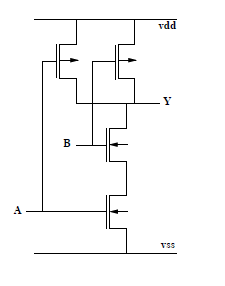
\includegraphics [scale = 1] {../figures/NAND}
 \caption{NAND schakeling m.b.v. NMOS en PMOS transistoren uit [1]}
 \label{res:NAND_schakeling}
 \end{center}
 \end{figure}

Een van de keerzijden van deze manier van schakelen, is het feit dat de NAND poort een bepaalde vertraging kent om het nieuwe signaal op de uitgang te zetten. Deze vertraging kan opgesplitst worden in twee gevallen. Enerzijds, wanneer het uitgangssignaal van hoog naar laag moet (T\tss{HL}) en anderzijds, wanneer het uitgangssignaal van laag naar hoog moet (T\tss{LH}). Deze vertraging kan worden beschreven aan de hand van een interne capaciteit van de NAND poort en een equivalente weer stand van de NAND poort.\\

Om de interne capaciteit te bepalen van de NAND poort zullen wij de capaciteit van het pull down netwerk bepalen,deze capaciteit is ten gevolge van T\tss{HL} . Om de capaciteit te bepalen van T\tss{HL} kan er gebruik worden gemaakt van het  circuit in figuur \ref{res:PDN_schakeling}, waarbij de beide ingangen gelijk zijn aan \emph{5V}. Het pull-up network (PUN) is dan dicht en het pull-down network (PDN) in geleiding. Deze capaciteit van het PDN wordt \emph{C\tss{out}}. Ook staat er een capaciteit parallel aan de NAND poort die de capaciteit van een eventuele load simuleert (\emph{C\tss{load} = 1pF}) die in de schakeling als C2 staat geschreven.


Verder wordt de vertragingstijd bepaal door de interne weerstand \emph{R\tss{eq}}  die op de interne weerstand van het PDN duidt.\\

Hoe deze capaciteit en weerstand kunnen worden gesimuleerd en berekend, wordt uitgelegd in hoofdstuk 4 Methode.

 \begin{figure} [h!]
 \begin{center}
 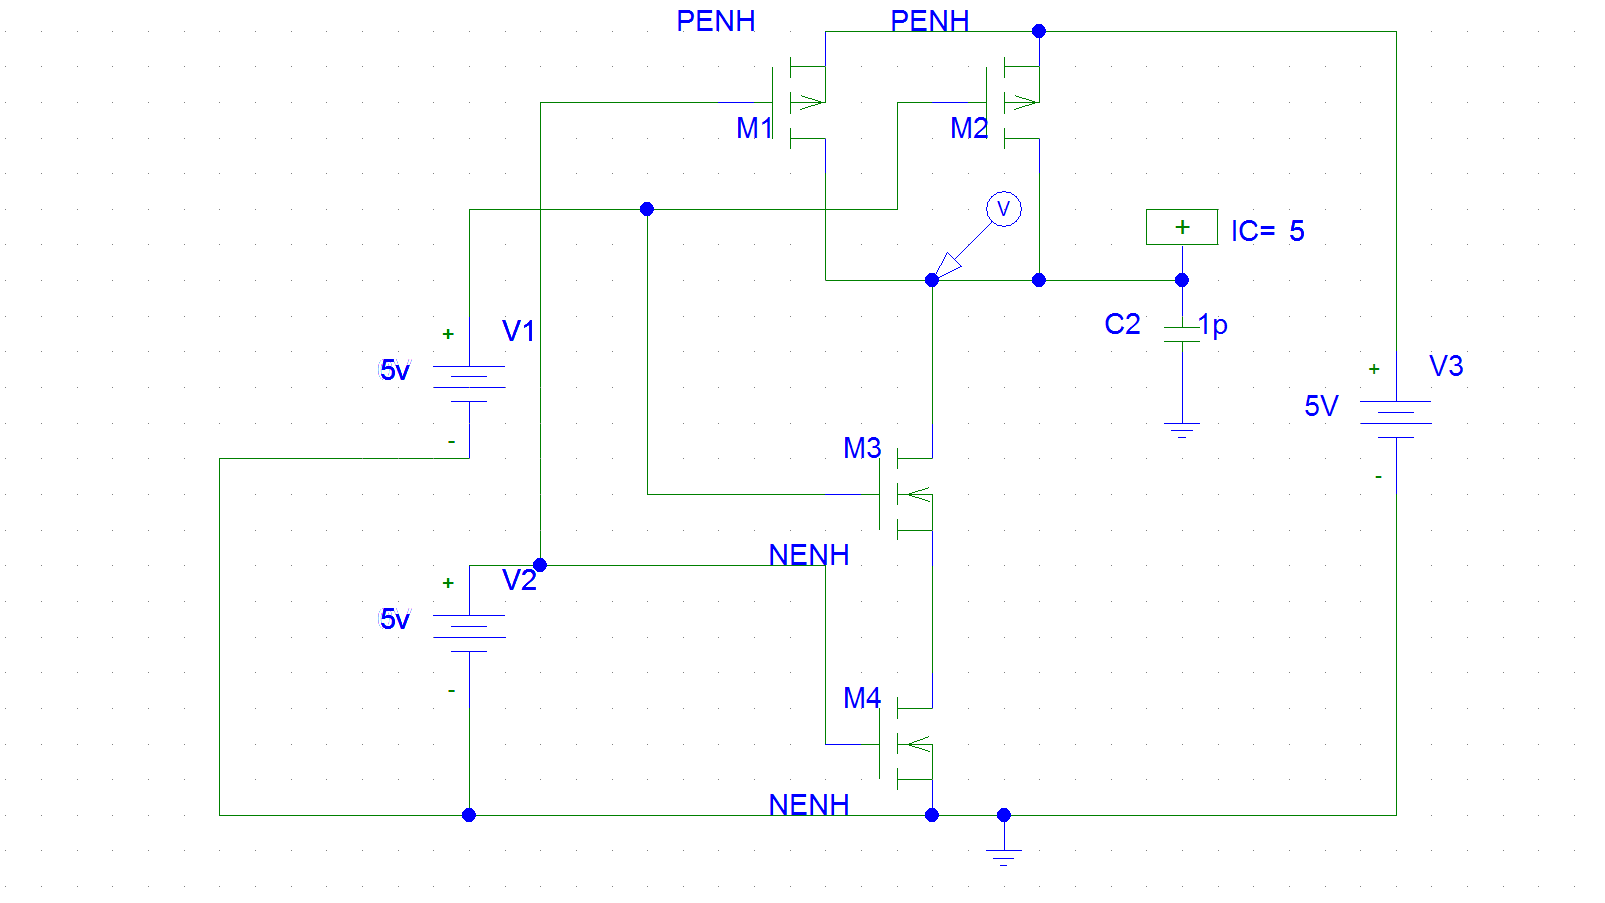
\includegraphics [scale = 0.4] {../figures/PDN}
 \caption{Simulatie opstelling voor het bepalen van \emph{C\tss{out,n} en R\tss{eq,n}}, de NENH en PENH zijn NMOS en PMOS transistoren, respectievelijk}
 \label{res:PDN_schakeling}
 \end{center}
 \end{figure}


\end{document}
